\chapter{实验}

\section{数据集介绍}
    本文进行实验的数据集来自 Khan Academy\footnote{https://www.khanacademy.org} 的教学视频及其相应的字幕文本和标签,
    这些教育视频涉及到多种学科和知识点,包括艺术、计算机科学、经济与金融、数学等。
    在表 \ref{table4.1} 中列出了该数据集的一些重要统计信息,同时在图 \ref{fig4.1} 中展示了视频标签与字幕长度的分布信息。
    Khan 数据集一共包括 7526 个不同的教育类视频,398 个不同的知识点标签。
    Khan 数据集的知识点标签体系为三层,平均每个教育视频的知识点标签个数为 3.76 个,平均每层的知识点标签个数分别为 1.14、1.41、1.21 个。
    同时可以看到,平均每个视频第二层的知识点标签个数反而大于第三层的知识点标签个数,这说明对 Khan 数据集中的教育类视频进行多标签知识点预测是一个不强制预测到最底层的任务。

    \renewcommand{\arraystretch}{1.2}
    \begin{table}[ht]
        \centering
        \begin{tabular}{c|c}
            % \specialrule{.1em}{.05em}{.05em}
            \toprule
            \makebox[0.5\textwidth][c]{\textbf{数据}} & \makebox[0.4\textwidth][c]{\textbf{数值}} \\
            \hline
            视频个数 & 7526 \\
            平均视频长度 & 432.13s \\
            平均字幕长度 & 1213.15 \\
            \hline
            知识点标签层数 & 3 \\
            第一层知识点个数 & 6 \\
            第二层知识点个数 & 42 \\
            第三层知识点个数 & 350 \\
            \hline
            平均每个视频知识点个数 & 3.76 \\
            平均每个视频第一层知识点个数 & 1.14 \\
            平均每个视频第二层知识点个数 & 1.41 \\
            平均每个视频第三层知识点个数 & 1.21 \\
            % \specialrule{.1em}{.05em}{.05em}
            \bottomrule
        \end{tabular}
        \caption{Khan 数据集统计信息}
        \label{table4.1}
    \end{table}
    \begin{figure}[htb]
        \centering
        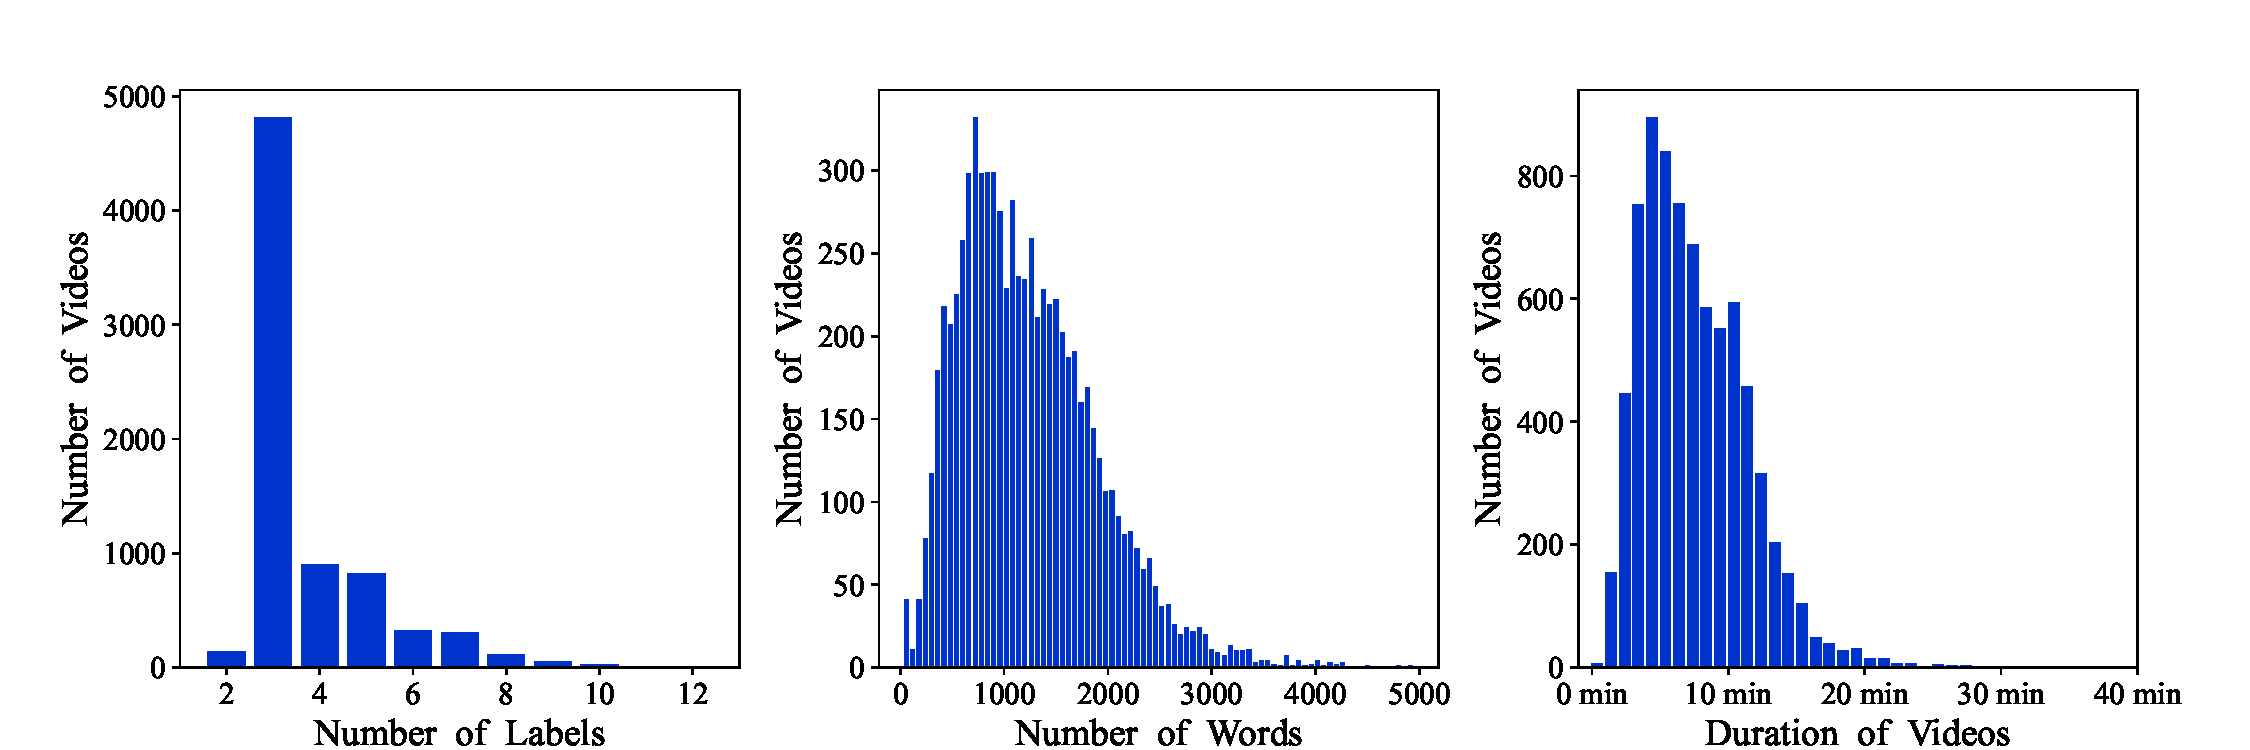
\includegraphics[width=1\linewidth]{Khan.pdf}
        \caption{Khan 数据集数据分布}
        \label{fig4.1}
    \end{figure}


\section{实验设置}
    \subsection{MKPN 参数设置}
    在实验中,对于模型本身的参数设置如下:

    本文使用 GloVe\cite{Pennington2014GloVeGV} 对字幕文本进行词嵌入,嵌入维度为 $100$ 维,同时设置双向 LSTM 层的隐藏维度为 $256$ 维。
    本文将所有从视频中提取出的关键帧的大小转化为 $224 \times 224$ 维,使用 ResNet34\cite{He2016DeepRL} 提取关键帧中的特征信息,每个关键帧会得到一个 $1000$ 维的特征向量。
    本文将标签嵌入的维度设置为 $200$ 维,同时使用 Xavier 初始化方法对所有标签的嵌入向量进行随机初始化。
    最后,本文将 HARL 中每一层输出的统一表征向量的维度设置为 $512$ 维。

    在模型训练过程中,本文设置的训练参数如下:

    本文在训练 MKPN 模型时使用 Adam\cite{Kingma2015AdamAM} 优化器对模型进行迭代更新,学习率设置为 $0.001$,每一步训练的 batch size 设置为 $8$。
    最后本文将用于权衡局部预测结果和全局预测结果的参数 $\alpha$ 设置为 $0.5$。

    \subsection{Baseline 方法}
    \subsubsection{HMCN-F\cite{Wehrmann2018HierarchicalMC}}
    HMCN-F 是一种使用混合预测方式来进行层级多标签分类的模型。该模型的主体结构为一系列全连接层,用于捕捉局部与全局的信息。
    本文在实验中只将字幕文本作为 HMCN-F 的输入。

    \subsubsection{HMCN-R\cite{Wehrmann2018HierarchicalMC}}
    HMCN-R 是 HMCN-F 的一种变体,主要区别在于主体结构从一系列全连接层变为类似于 LSTM 的循环网络。HMCN-R 同样使用混合预测的方式来同时获取局部和全局信息。
    本文在实验中只将字幕文本作为 HMCN-F 的输入。

    \subsubsection{ResNet + TextCNN\cite{He2016DeepRL, Kim2014ConvolutionalNN}}
    在该 Baseline 方法中,本文分别使用 ResNet 和 TextCNN 对视频和字幕文本进行特征提取,然后将这两部分特征进行简单拼接,使用全局预测的方式来进行知识点预测。

    \subsubsection{MKPN-Text}
    MKPN-Text 是 MKPN 的一种变体,本文在该变体中仅用字幕文本作为模型的输入,而忽略来自视频的信息。

    \subsubsection{MKPN-G}
    MKPN-G 是 MKPN 的一种变体,本文在该变体中忽略局部预测结果,而仅使用全局预测的方式来进行知识点预测。

    \subsubsection{MKPN-L}
    MKPN-L 是 MKPN 的一种变体,本文在该变体中忽略全局预测结果,而仅使用局部预测的方式来进行知识点预测。

    以上各 Baseline 与 MKPN 模型在多模态信息的使用和层级多标签预测上的特点如表 \ref{table4.2} 所示。

    \renewcommand{\arraystretch}{1.2}
    \begin{table}[ht]
        \centering
        \begin{tabular}{c|cccc}
            % \specialrule{.1em}{.05em}{.05em}
            \toprule
            \multirow{2}{*}{\makebox[0.3\textwidth][c]{\textbf{Baseline}}} & \multirow{2}{*}{\makebox[0.2\textwidth][c]{\textbf{Multimodal}}} & \multicolumn{3}{c}{\makebox[0.3\textwidth][c]{\textbf{Method}}} \\
            \cline{3-5}
            & & Local & Global & Hybrid \\
            \hline
            HMCN-R & - & - & - & \checkmark \\
            HMCN-F & - & - & - & \checkmark \\
            ResNet + TextCNN & \checkmark & - & - & - \\
            MKPN-Text & - & - & - & \checkmark \\
            MKPN-L & \checkmark & \checkmark & - & - \\
            MKPN-G & \checkmark & - & \checkmark & - \\
            MKPN & \checkmark & - & - & \checkmark \\
            % \specialrule{.1em}{.05em}{.05em}
            \bottomrule
        \end{tabular}
        \caption{各模型特点}
        \label{table4.2}
    \end{table}


\section{评价指标}
    \subsection{准确率、召回率和 F1 值}
    考虑到对教学资源进行知识点预测本质上是层级多标签分类任务,因此本文使用在多标签分类领域中被广泛应用的指标来对实验结果进行评价:准确率(precision),召回率(recall)和 F1 值。
    在实验中,若一个知识点标签的最终预测分数不小于阈值,则认为模型将该知识点标签标记为正。本文在实验中设置阈值 threshold\ =\ 0.5。
    对于知识点体系中的每一个知识点 $i \in K$,记 $TP_i$ 为知识点 $i$ 在真实标签中且被模型预测为正的次数,
    $FP_i$ 为知识点 $i$ 不在真实标签中但被模型预测为正的次数,$FN_i$ 为知识点 $i$ 在真实标签中但被模型预测为负的次数,则准确率和召回率的计算方式如下:
    \begin{equation}
        \begin{aligned}
            &precision = \dfrac{\sum_{i \in K}TP_i}{\sum_{i \in K}TP_i + \sum_{i \in K}FP_i} \\
            &recall = \dfrac{\sum_{i \in K}TP_i}{\sum_{i \in K}TP_i + \sum_{i \in K}FN_i}
        \end{aligned}
    \end{equation}
    同时,为了更便于同时比较准确率和召回率,本文还使用 Micro-F1 值来衡量不同模型的效果。Micro-F1 为准确率和召回率的调和平均值:
    \begin{equation}
        Micro-F1 = \dfrac{2 * precision * recall}{precision + recall}
    \end{equation}
    准确率、召回率、Micro-F1 值越大,代表模型的知识点预测效果越好。

    % \subsection{AUPRC}
    % AUPRC 即为准确率-召回率曲线与坐标轴围成为面积值。AUPRC 也是一个用于综合衡量准确率和召回率的指标,与 F1 值不同的是,AUPRC 的计算过程避免了阈值的设置。
    % 由于为知识点预测分数选择不同的阈值会得到不同的 F1 值,为了避免阈值的选取对不同模型的预测指标的影响,我们再使用 AUPRC 对不同模型的综合预测性能进行评价。
    % 与 F1 值类似,AUPRC 值越高,表示对应模型的知识点预测效果越好。

\section{实验结果}
    \subsection{模型效果比较}
    所有 Baseline 与 MKPN 模型在 Khan 数据集上的知识点预测结果在表 \ref{table4.3} 中列出。
    可以看到 MKPN 模型在 Khan 数据集上取得了综合最好的知识点预测效果,这说明了 MKPN 模型在对于教育类视频进行知识点预测时具有良好的多模态信息捕捉能力,以及利用知识点层级结构进行层级分类的能力。
    同时可以注意到,能够利用多模态信息的模型在综合预测能力上都要优于使用单模态进行预测的模型。
    这一点尤其体现在各模型对于知识点的召回率上,未结合使用多模态信息的模型在进行知识点预测时的召回率要明显更低,这说明仅使用文本信息的模型对于视频中的特征信息提炼效果不佳,
    从而证明了在对教育类视频进行知识点预测时结合多模态信息的必要性。

    \renewcommand{\arraystretch}{1.2}
    \begin{table}[ht]
        \centering
        \begin{tabular}{c|c|c|c}
            % \specialrule{.1em}{.05em}{.05em}
            \toprule
            \multirow{2}{*}{\makebox[0.3\textwidth][c]{\textbf{Baseline}}} & \multicolumn{3}{c}{\makebox[0.6\textwidth][c]{\textbf{Metrics}}} \\
            \cline{2-4}
             & \makebox[0.2\textwidth][c]{\textbf{Precision}} & \makebox[0.2\textwidth][c]{\textbf{Recall}} & \makebox[0.2\textwidth][c]{\textbf{Micro-F1}} \\
            \hline
            HMCN-R & 0.8834 & 0.3329 & 0.4836 \\
            HMCN-F & 0.8286 & 0.4946 & 0.6194 \\
            ResNet + TextCNN & 0.8397 & 0.5266 & 0.6473 \\
            MKPN-Text & 0.8642 & 0.4860 & 0.6221 \\
            MKPN-L & 0.7393 & 0.5865 & 0.6541 \\
            MKPN-G & 0.7146 & \textbf{0.6427} & 0.6767 \\
            MKPN & \textbf{0.8916} & 0.5532 & \textbf{0.6828} \\
            \bottomrule
        \end{tabular}
        \caption{各模型知识点预测性能(基于内容抽取关键帧)}
        \label{table4.3}
    \end{table}

    \subsection{MKPN 变体模型比较}
    从表 \ref{table4.3} 中可以看出 MPKN 模型相较于其他 MPKN 变体而言综合预测效果更好。
    仅使用了文本信息的 MKPN-Text 在所有 MKPN 变体中的综合预测效果最差,知识点召回率远低于其他变体,这进一步说明多模态学习对于教育类视频的重要性。
    与此同时,可以看到相较于使用了混合预测模式的 MKPN 与 MKPN-Text,仅通过局部预测或全局预测方式的 MKPN-L 和 MKPN-G 在预测准确率上很低,而预测召回率较高,
    这说明 MKPN-L 和 MKPN-G 更倾向于预测更多的知识点,但不能较好地保证所预测知识点的正确率。
    而 MKPN 模型能够通过结合局部预测和全局预测这两种方式来对预测结果进行精选,仅有当一个知识点在局部预测和全局预测中都具有较高的预测分数时,MKPN 模型才会将该知识点标记为正进行输出,
    一定程度上避免了模型预测时的偶然性,从而能够提高预测时的准确率,但同时也会对召回率造成一定影响。

    \begin{figure}[htb]
        \centering
        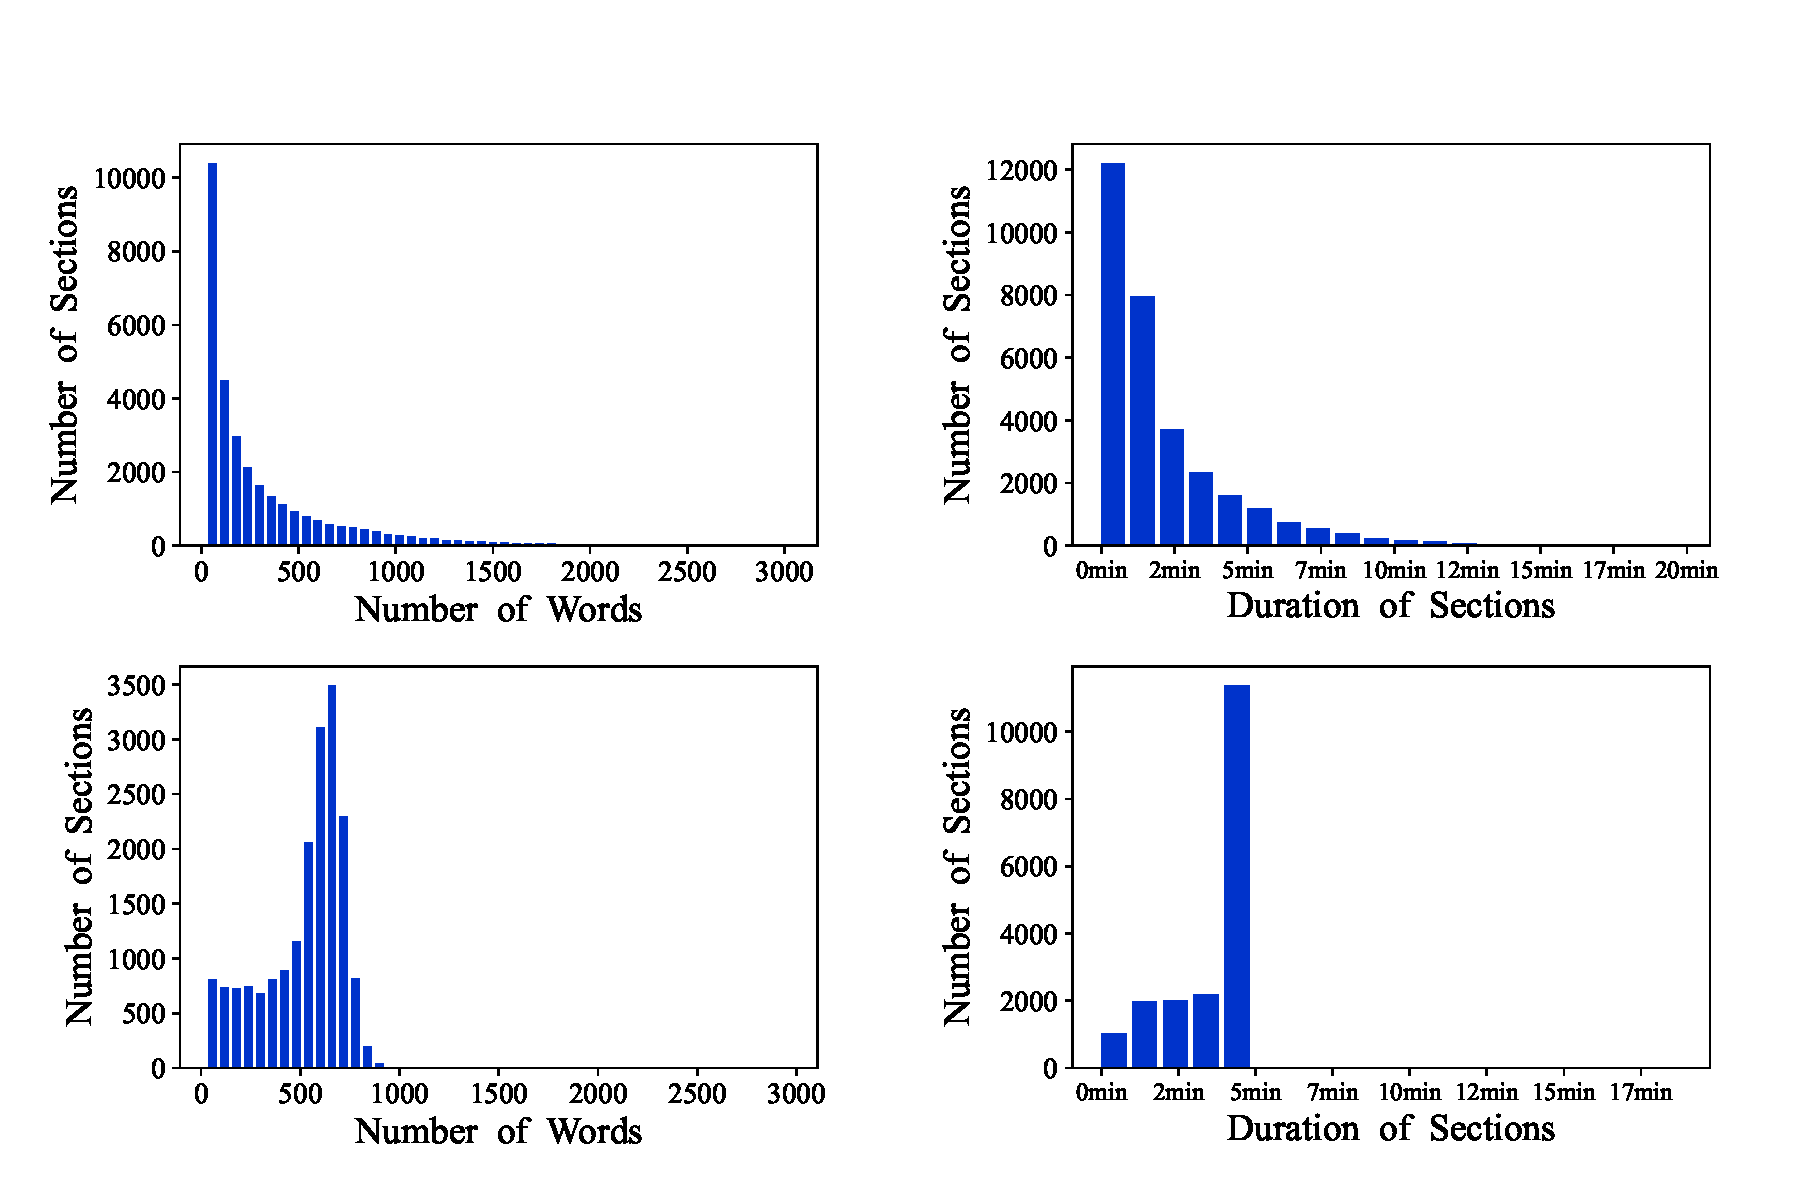
\includegraphics[width=1\linewidth]{section-distribution.pdf}
        \caption{视频块时长和字幕长度分布}
        \label{fig4.2}
    \end{figure}

    \subsection{视频关键帧抽取效果比较}
    为了说明本文对教育类视频进行关键帧抽取和视频分块方式的合理性,这里使用一个更为简单的关键帧抽取算法对 Khan 数据集进行处理。
    考虑到 Khan 数据集视频平均长度为 432 秒,本文通过时长对视频进行分块,将所有视频都切割为一系列最长时长不超过 200 秒的视频块,每个视频块的首尾两帧作为该视频块的关键帧。
    将本文提出的根据内容进行关键帧抽取的算法和根据时长进行关键帧抽取的算法在 Khan 数据集上分别进行实验,得到的视频块分布信息如图 \ref{fig4.2} 所示。
    各模型在经基于时长的关键帧抽取算法处理后的 Khan 数据集中进行知识点预测的效果列在表 \ref{table4.4} 中,同时与表 \ref{table4.3} 的对比结果展示在图 \ref{fig4.3} 中。
    从图 \ref{fig4.3} 中可以看到各模型的预测召回率有普遍的降低。
    这说明不考虑视频内容而简单地根据时长进行切割会导致一定程度的视频信息割裂,从而引起模型对割裂部分信息提取效果不佳,最终可能使得模型对割裂部分的知识点预测产生遗漏。
    相较而言,本文基于视频内容对教育类视频进行关键帧抽取和视频分块能够更好地保证每一个视频块的内容完整性,因此证明了本文基于视频内容的关键帧抽取算法的合理性。

    \renewcommand{\arraystretch}{1.2}
    \begin{table}[ht]
        \centering
        \begin{tabular}{c|c|c|c}
            % \specialrule{.1em}{.05em}{.05em}
            \toprule
            \multirow{2}{*}{\makebox[0.3\textwidth][c]{\textbf{Baseline}}} & \multicolumn{3}{c}{\makebox[0.6\textwidth][c]{\textbf{Metrics}}} \\
            \cline{2-4}
             & \makebox[0.2\textwidth][c]{\textbf{Precision}} & \makebox[0.2\textwidth][c]{\textbf{Recall}} & \makebox[0.2\textwidth][c]{\textbf{Micro-F1}} \\
            \hline
            HMCN-R & \textbf{0.8827} & 0.3056 & 0.4540 \\
            HMCN-F & 0.8400 & 0.4772 & 0.6087 \\
            ResNet + TextCNN & 0.8526 & 0.5198 & 0.6458 \\
            MKPN & 0.8599 & \textbf{0.5352} & \textbf{0.6598} \\
            \bottomrule
        \end{tabular}
        \caption{各模型知识点预测性能(基于时长抽取关键帧)}
        \label{table4.4}
    \end{table}

    \begin{figure}[htb]
        \centering
        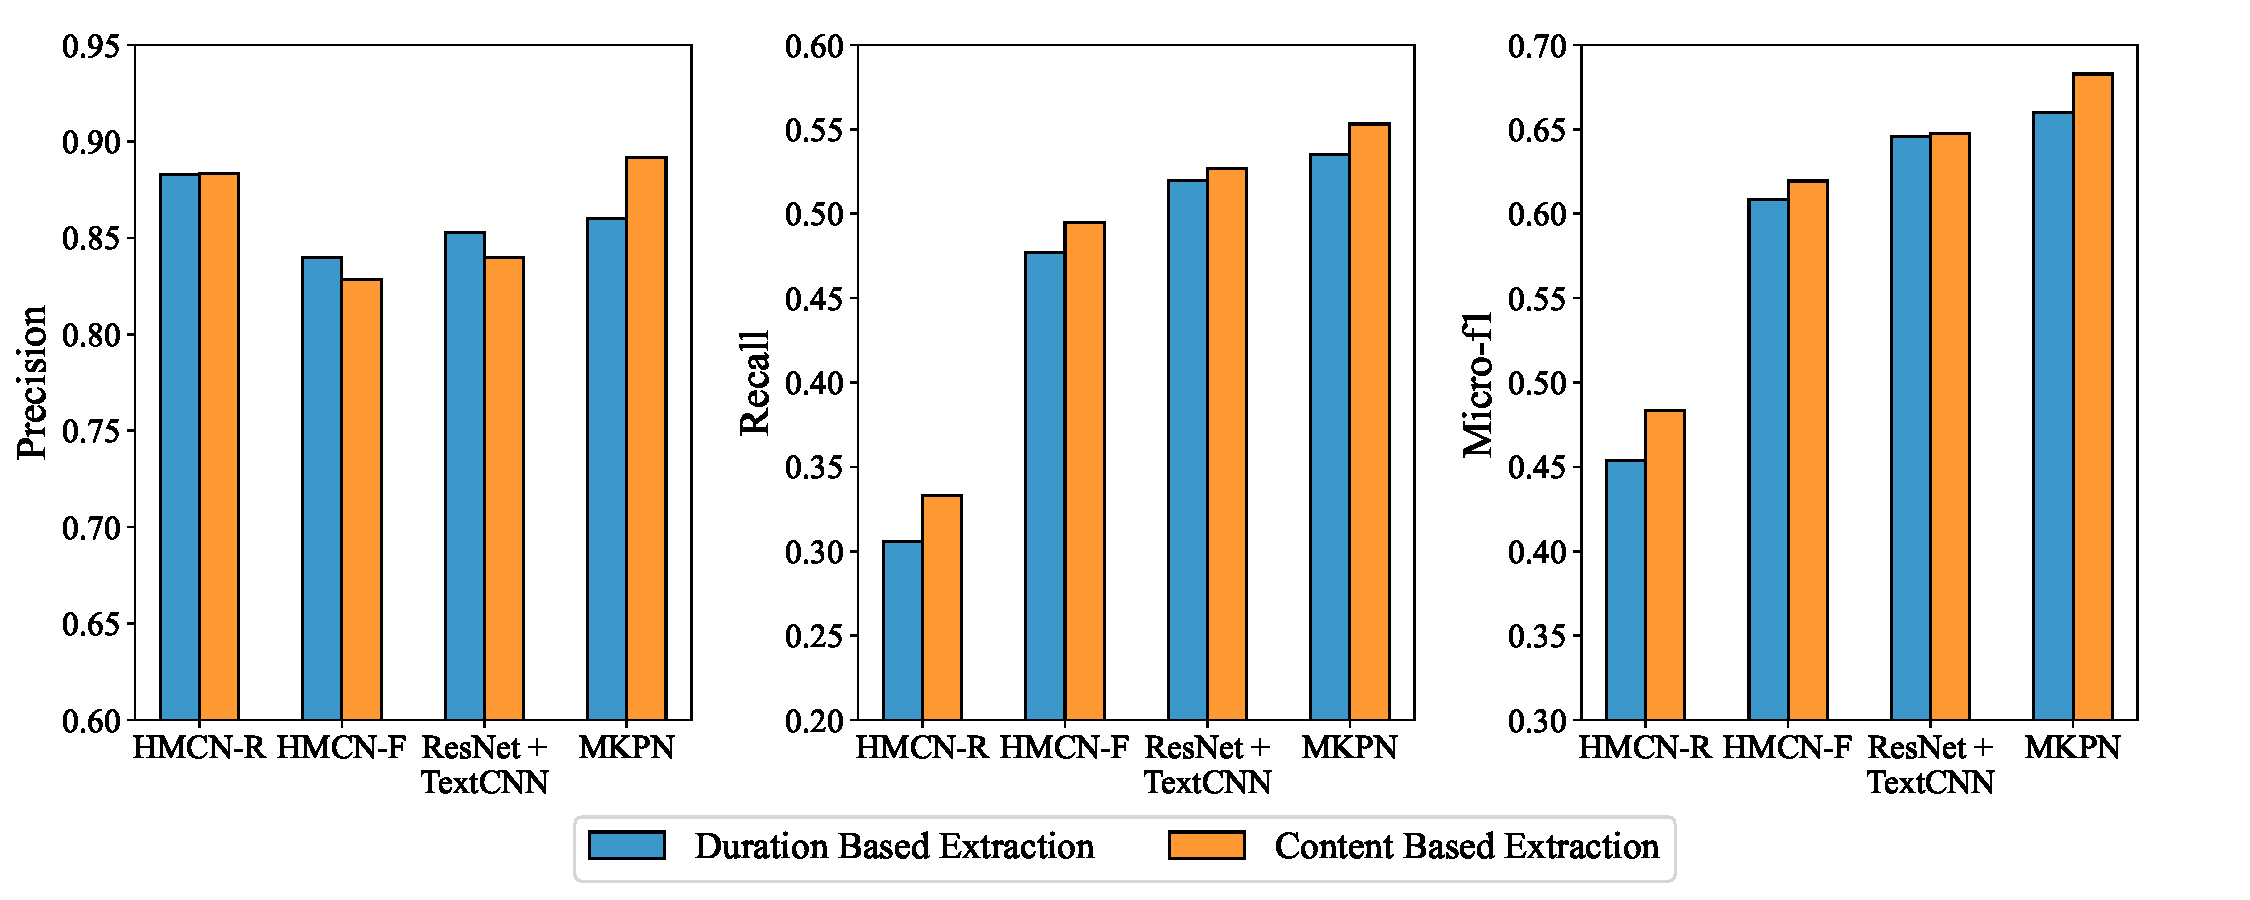
\includegraphics[width=1\linewidth]{performance-comparation.pdf}
        \caption{基于不同关键帧抽取算法的各模型性能比较}
        \label{fig4.3}
    \end{figure}
